\chapter{Introduction}
\label{sec:introduction}

The future of robotic systems trends towards autonomous operations in unstructured environments.
Thereby, reliable and dynamically accurate motion planning is a fundamental requirement for the operation 
of robotic systems. Essential applications are search and rescue operations, naturally hazardous to humans,
in which especially legged robots have the potential to gain access and precisely navigate 
through complex terrain (see Figure~\ref{fig:introduction_applications_legged}) 
\cite{LIU}. 
But also in industrial contexts, robots assembling various components require careful and 
precise motion planning. For example,
Figure~\ref{fig:introduction_applications_kuka} illustrates a thermal processing application
\cite{Intro_KUKA}. 
Both applications consist of different tasks and 
constraints. However, both systems pose the same fundamental problem. 
Several rigid bodies must be moved from an initial configuration to a desired configuration by
admissible control inputs, while their rotations, joint connections, nonlinear
dynamics, and actuator limits must be satisfied simultaneously. Thereby,
generated trajectories can be restricted to avoid collisions, while being dynamically feasible \cite{Kang_2025Global}.

\begin{figure}[tb]
    \centering
    \subfigure[Legged locomotion]{
        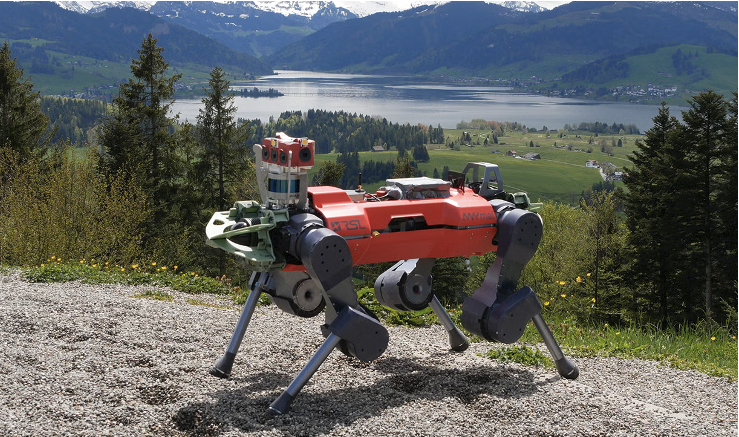
\includegraphics[width=0.47\textwidth]{pics/Introduction/Legged_Robot_high_resolution.pdf}
        \label{fig:introduction_applications_legged}
    }
    \hfill
    \subfigure[Industrial robot]{
        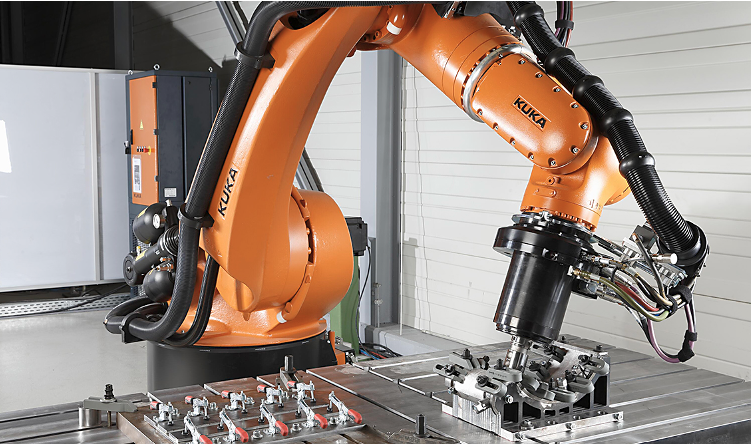
\includegraphics[width=0.47\textwidth]{pics/Introduction/KUKA_high_resolution.pdf}
        \label{fig:introduction_applications_kuka}
    }
    \caption{Examples of robotic systems composed of coupled rigid bodies: (a) legged
    locomotion taken from \cite{Intro_Legged} and (b) industrial manipulation taken from \cite{Intro_KUKA}.}
    \label{fig:introduction_applications}
\end{figure}

In addition to a large number of system variables, rigid-body attitudes
belong to rotation groups, considered as Lie groups, rather than to a Euclidean vector
space. Joint constraints couple the configuration of neighbouring bodies, and the
equations of motion couple states and controls over time \cite{Sangli2025}. Consequently, even a
finite-horizon problem without contact or obstacles generally contains nonlinear
equalities and nonconvex rotation constraints. Its feasible set can have several
disconnected regions, and its objective can contain many local minima \cite{Kang_2026Fast}.
Moreover, the continuous-time dynamics are high dimensional as state and control trajectories
are functions of time. So any numerical
solution must discretize these problems. Nevertheless, classic global optimization methods simplify
the dynamics of robotic systems by approximating them with simpler models \cite{Sangli2025}. 
Thereby, the discrete dynamics can differ from the continuous dynamics through 
loss of geometric structure and manifold drift, 
which results in deviations from the true solution and 
numerical infeasibility \cite{Marsden2001}.

Currently, nonlinear programming is one of the most common approaches for computing robot 
trajectories. Starting from an initial guess, these methods repeatedly adjust the states and 
control inputs to find a trajectory with a low objective value that satisfies the given 
constraints \cite{Betts1998TrajectoryOptimization,tedrake_underactuated}. Sequential convex 
methods, such as TrajOpt, follow a similar idea but replace the original difficult problem 
with a sequence of simpler convex problems \cite{Schulman2014TrajOpt}. Both approaches can 
find useful motions efficiently, even for relatively large robot models. However, the final 
result may depend strongly on the initial guess and is generally only locally optimal.
Sampling-based methods instead explore many possible configurations and connect them to 
construct a path. Although some of these methods are asymptotically optimal, a path obtained 
after a finite computation does not provide a certificate of global optimality 
\cite{KaramanFrazzoli2011Sampling}.

To address the limitations of local methods, this thesis investigates semidefinite 
programming (SDP) for multibody systems. An SDP is a convex optimization problem formulated
using matrix variables. Instead of solving the original nonconvex motion-planning problem directly, a semidefinite 
relaxation constructs a convex approximation that can be solved reliably and provides a lower 
bound on the globally optimal objective value \cite{VandenbergheBoyd1996SDP,Lasserre2001Global}. 
In contrast, a feasible trajectory, for example generated by a local optimization method
such as NLP or TrajOpt, provides an upper bound. 
If the suboptimality gap between the SDP lower bound and the feasible-trajectory 
upper bound is within the specified numerical tolerance, the trajectory is \emph{certified} 
as globally optimal for the considered discrete motion-planning problem \cite{Sangli2025}.

However, realistic trajectory optimization also requires a discrete model that represents
the rigid-body dynamics accurately. Lie group variational integrators (LGVIs) discretize the 
equations of motion directly on the configuration manifold and update rotations through the 
Lie-group structure \cite{Marsden2001,Lee2008}. Consequently, the numerical rotations remain 
on the rotation group. LGVIs also preserve important 
geometric properties of the mechanical system, such as its symplectic structure and 
energy conservation over a long time duration \cite{Sangli2025}. 

Therefore, the key idea of this thesis is to combine these two approaches. For the considered 
rigid-body systems, the LGVI dynamics can be expressed through low-degree polynomial equations. 
The resulting polynomial motion-planning problem can then be approximated by a Moment--SOS 
semidefinite relaxation \cite{Sangli2025}. Thereby, the LGVI provides a structure-preserving 
model of the rigid-body dynamics, while the SDP provides a global lower bound and 
certifies global optimality.
This is the case when the relaxation is tight and a feasible trajectory can be extracted. 
The complete 
concept is summarized in Figure~\ref{fig:intro_pipeline}.

\begin{figure}[t!]
    \centering

    \begin{tikzpicture}[
        >=Latex,
        node distance=5mm,
        block/.style={
            rounded corners=1.5mm,
            draw=black!45,
            fill=black!2,
            thick,
            align=center,
            text width=8.8cm,
            minimum height=0.75cm,
            font=\small
        },
        titled/.style={
            rectangle split,
            rectangle split parts=2,
            rectangle split part align={left,center},
            rounded corners=2mm,
            line width=1pt,
            text width=9cm,
            inner xsep=2mm,
            inner ysep=1mm,
            font=\small
        },
        arrow/.style={
            -{Latex[length=2.2mm]},
            thick,
            draw=black!65
        }
    ]

    % Main problem
    \node[
        titled,
        draw=tum_blue,
        rectangle split part fill={
            tum_blue,
            tum_blue!8!white
        }
    ] (problem)
    {
        \textcolor{white}{\figureboxtitle{Main Problem}}
        \nodepart{second}
        Nonlinear and nonconvex rigid-body trajectory optimization
    };

    \node[
        block,
        below=7mm of problem
    ] (lgvi)
    {
        Lie group variational discretization\\[-1mm]
        \scriptsize structure-preserving rigid-body dynamics
    };

    \node[
        block,
        below=of lgvi
    ] (pop)
    {
        Polynomial motion-planning formulation
    };

    \node[
        block,
        below=of pop
    ] (sdp)
    {
        Sparse Moment--SOS semidefinite relaxation\\[-1mm]
        \scriptsize convex global lower bound
    };

    % Key idea
    \node[
        titled,
        draw=tum_orange,
        rectangle split part fill={
            tum_orange,
            orange!8!white
        },
        below=7mm of sdp
    ] (idea)
    {
        \textcolor{white}{\figureboxtitle{Key Idea}}
        \nodepart{second}
        Structure-preserving LGVI dynamics combined with
        semidefinite relaxation
    };

    \draw[arrow] (problem) -- (lgvi);
    \draw[arrow] (lgvi) -- (pop);
    \draw[arrow] (pop) -- (sdp);
    \draw[arrow] (sdp) -- (idea);

    \end{tikzpicture}

    \caption{Framework of this thesis.
    Lie group variational discretization provides structure-preserving
    rigid-body dynamics, while sparse semidefinite relaxation provides
    a convex lower bound for the resulting polynomial motion-planning
    problem.}
    \label{fig:intro_pipeline}
\end{figure}

This thesis investigates a 3D pendulum as a 
single-rigid-body system and an Acrobot as a constrained and underactuated multibody system. 
The main contributions of this thesis are:

\begin{itemize}
\item The explanation of an LGVI for the controlled and unforced 3D pendulum on $\mathrm{SO}(3)$, 
providing a structure-preserving discrete model of a single rigid body.

\item The derivation of a constrained LGVI for the Acrobot in maximal coordinates on 
$(\mathrm{SO}(2)\times \mathbb{R}^2)^2$.
Thereby, the positions and rotations of both rigid links are represented separately 
and connected through holonomic joint constraints.

\item The numerical implementation and validation of both LGVI models, including the 
preservation of the rotation and joint constraints, and the conserved long-term energy 
behavior.

\item The formulation of the 3D-pendulum polynomial optimization problem (POP) as a polynomial 
optimization problem and its solution through a sparse Moment-SOS semidefinite relaxation. 
This is followed by an assessment of relaxation tightness, extraction feasibility, and the availability 
of global-optimality certificates.

\item The formulation of the Acrobot POP using a reduced polynomial 
model, problem-specific sparse SDP structures and its solution through 
a sparse Moment-SOS semidefinite relaxation.
Finally, the evaluation of the extracted trajectories and their global optimality certificates.
Thereby, the evaluation is extended to a closed-loop implementation.
\end{itemize}

\section{Problem Statement}
\label{sec:introduction_problem_statement}

The framework illustrated in Figure \ref{fig:intro_pipeline} addresses the
following general motion planning problem. Thereby, the objective is to optimize the path 
of a rigid-body system from
an initial configuration towards a desired configuration, while respecting the system's
dynamics, geometric structure, joint connections, and physical limits.
The motion is considered over a finite horizon divided into $N$ intervals. Let $\bm{Y}_k$ describe
the configuration and discrete motion of the system at step $k$, let $\bm{U}_k$ denote
the applied control input, and let $\bm{\lambda}_k$ contain joint-constraint multipliers
when several bodies are connected. The rigid links are indexed by
$i\in\mathcal B:=\{1,\ldots,n_{\mathrm b}\}$. At a high level, the corresponding
motion-planning problem can be written as
\begin{subequations}
\label{eq:problem_statement}
\begin{align}
p^\star =
\min_{\{\bm{Y}_k\}_{k=0}^{N},\{\bm{U}_k,\bm{\lambda}_k\}_{k=1}^{N}}
\quad & \Psi(\bm{Y}_N)+\sum_{k=0}^{N-1}\psi(\bm{Y}_k,\bm{U}_{k+1},\bm{\lambda}_{k+1}),
\label{eq:problem_statement_objective}\\
\text{s.t.}\quad
&\bm{Y}_0=\bm{Y}_{\mathrm{init}},
\label{eq:problem_statement_initial}\\
&\mathcal D_i(\bm{Y}_{k+1},\bm{Y}_k,\bm{U}_{k+1},\bm{\lambda}_{k+1})=0,
\label{eq:problem_statement_dynamics}\\
&(\bm{Y}_{k+1}, \bm{Y}_k,\bm{U}_{k+1},\bm{\lambda}_{k+1})\in\mathcal{A}_k,
\label{eq:problem_statement_admissible}
\end{align}
\end{subequations}

for $k=0,\ldots,N-1$. The objective combines the terminal cost $\Psi$ with the running cost $\psi$. Additionally, the
constraints $\mathcal D_i=0$ represent the discrete rigid-body dynamics of link $i$.
For this compact statement, the admissible set $\mathcal A_k$ collects the Lie-group constraints,
inequality constraints, and control bounds that are written separately as
$\mathcal Y_i$, $\mathcal H$, and $\bm{U}_{\min}\leq \bm{U}_{k+1}\leq \bm{U}_{\max}$ in
Chapter~\ref{chapter:certifiable_trajectory_optimization}. Therefore, \eqref{eq:problem_statement}
summarizes the physical requirements of the problem, generalizing it to any robotic system \cite{Kang_2026Fast}. 

Generally, the objective appears simple. However, for many robotic systems composed of many rigid bodies, 
the equality constraints $\mathcal D_i$ are nonlinear, and
the rotation constraints and equations of
motion make the feasible set nonconvex. The LGVI formulation is useful because the
considered dynamics can be expressed by low-degree
polynomials and have energy-conservation properties \cite{Sangli2025}. 
After collecting all scalar decision variables in
$\bm{z}\in\mathbb{R}^{n_z}$, \eqref{eq:problem_statement} takes the standard
polynomial form
\begin{equation}
\label{eq:problem_statement_polynomial_form}
p^\star=\min_{\bm{z}\in\mathbb{R}^{n_z}}p(\bm{z})
\quad\text{s.t.}\quad
h_i(\bm{z})=0,\ i\in\mathcal{E},
\qquad
g_j(\bm{z})\geq0,\ j\in\mathcal{J},
\end{equation}
\cite{Yang2024Semidefinite}. Here, $p^*$ is the globally optimal value, $h_i$ are polynomial equality constraints,
and $g_j$ are polynomial inequality constraints, with their respective sets $\mathcal{E}$ and $\mathcal{J}$.
This polynomial optimization problem remains nonconvex. At a selected relaxation
order $\kappa$, a Moment-SOS semidefinite relaxation replaces \eqref{eq:problem_statement_polynomial_form}
by a convex problem and returns a global lower bound $\gamma_\kappa^\star$. In contrast, every
verified feasible trajectory $\hat{\bm{z}}$ provides an upper bound through its objective
value. Therefore, the globally optimal value $p^\star$ of the objective is bounded by
\begin{equation}
\label{eq:problem_statement_bounds}
\gamma_\kappa^\star\leq p^\star\leq p(\hat{\bm{z}}).
\end{equation}
If the lower and upper bounds agree within specified numerical tolerances, the
feasible trajectory is certified as globally optimal \cite{Lasserre2001Global}.

Therefore, the central research question of this thesis is as follows:

\begin{quote}
\emph{What are the capabilities and limitations of combining structure-preserving Lie group variational 
integrators with semidefinite relaxation to obtain feasible and certifiably 
optimal trajectories for single- and multi rigid-body systems?}
\end{quote}

This question is investigated by first deriving structure-preserving LGVI models,
then formulating the resulting discrete dynamics as polynomial optimization
problems, and finally evaluating the SDP relaxations in terms of feasibility,
tightness, certifiability, and computational cost.

\section{Related Work}
\label{sec:introduction_related_work}

\paragraph{Trajectory optimization and global planning}

Trajectory optimization represents a robot motion by a finite sequence of states
and control inputs. Direct nonlinear programming methods are widely used
because they can solve large problems efficiently, described in
\cite{Betts1998TrajectoryOptimization,tedrake_underactuated}. Sequential convex
methods such as TrajOpt, from \cite{Schulman2014TrajOpt}, similarly replace the original problem by a sequence of
simpler subproblems. These approaches can produce useful
motions fast, but generally converge only to a local solution and therefore
depend on the initial guess. Sampling-based planners such as PRM$^*$ and RRT$^*$
offer asymptotic optimality, but not a global certificate after a finite computation
\cite{KaramanFrazzoli2011Sampling}. Mixed-integer formulations of 
\cite{DeitsTedrake2014Footstep,DaiIzattTedrake2019IK} provide global
statements for selected problems such as footstep placement and inverse kinematics,
although their computational cost and model approximations are inefficient for
general multibody dynamics.
\cite{Posa2014Contact,Manchester2019ContactVI}.
investigated contact-implicit methods
by including contact forces and mode changes directly in the optimization.

\paragraph{Geometric mechanics and variational integration}

Rigid-body attitudes naturally belong to Lie groups rather than Euclidean vector
spaces. The required foundations of Lie groups, mechanical symmetry, rigid-body
mechanics, inertia, and matrix analysis are provided in
\cite{Hall2000LieGroups,MarsdenRatiu1999,Benacquista2018ClassicalMechanics,
RITInertiaTable216,GallierQuaintance2020LinearAlgebra,YanaiTakeuchiTakane2011SVD}.
Classical integration methods are summarized by Butcher
\cite{butcher2016numerical}, whereas geometric integration emphasizes the
preservation of mechanical structure over long simulations
\cite{Hairer1994,Leimkuhler_Reich_2005}. Projection can restore manifold
constraints after a numerical step \cite{Hairer2000}, while Lie-group integrators
update the configuration directly on the group \cite{CELLEDONI2003421}.
Retraction maps such as the Cayley transform provide a
computational implementation of the implicit Lie-group update, described in
\cite{Arieh_Cayley_Motivation,ColomboJimenez2012SO3_Cayley,
Barbero-Linan2023_Cayley_Formula}.

Variational integrators derive the discrete equations of motion from a discrete
action principle and thereby preserve important geometric properties of the
continuous mechanics, which are defined in \cite{Marsden2001}. 
\cite{Lee2008} develops this approach directly on
matrix Lie groups and applies it to rigid-body mechanics, optimal control, and the
full-body problem. The approach is extended in
\cite{Lee2007,LeeLeokMcClamroch2007DiscreteControlSystems}. The 3D pendulum
provides a compact benchmark for these rotational dynamics \cite{Shen20043DPendulum}.
For multibody systems, maximal coordinates assign a pose to every body and impose
joints through algebraic constraints, defined in 
\cite{BrudigamManchester2021VariationalIntegrators,BrudigamManchester2021LQR}.
These works form the basis for the 3D-pendulum and maximal-coordinate Acrobot LGVIs
derived in this thesis.

\paragraph{Polynomial optimization and sparse semidefinite relaxation}

Semidefinite programming is a convex optimization framework
\cite{VandenbergheBoyd1996SDP}. Moment-SOS methods use it to relax polynomial
optimization problems and obtain global lower bounds. 
\cite{Putinar1993Positive,Lasserre2001Global,Yang2024Semidefinite} establish their 
theoretical basis is
given by positivity certificates and the Lasserre hierarchy. However,
tightness at a selected relaxation order is not guaranteed, as discussed in
\cite{Nie2014FiniteConvergence}. Dense moment matrices grow rapidly with the number
of variables. Correlative sparsity instead constructs smaller overlapping matrices
and can preserve convergence under suitable conditions given in
\cite{Waki2006Sparse,Lasserre2006Sparse}.

\cite{Sangli2025} combine Lie-group variational integrators with sparse moment relaxation
for multibody motion planning and therefore provide the closest methodological
foundation for this thesis. \cite{Kang_2026Fast} show that specialized
sparse formulations and first-order GPU solvers can substantially accelerate
certifiable trajectory optimization. \cite{Kang_2025Global} extend sparsity-rich
relaxations to contact-rich planning. These developments
demonstrate the potential of the approach, while also showing that relaxation size
and solver choice remain decisive. This thesis uses the interior-point solver MOSEK
for optimization \cite{MOSEK}.
Related SDP-based MPC research further illustrates the relevance of repeatedly
solving relaxations in closed loop, as shown in \cite{Hartmann_2026SDP}. The implementation and
experiments presented in this thesis are documented in the open-source
repository \cite{Elshani2026CTO_GitHub}.

\section{Research Gap}
\label{sec:introduction_research_gap}

The connection between LGVIs and semidefinite relaxation has already
been investigated in recent works. However, it does not provide certifiably optimal trajectories for every
problem. \cite{Sangli2025} combines LGVIs with sparse Moment-SOS relaxations for
single- and multibody systems. Still, some relaxations are not
tight, requiring the extracted solutions to be refined using nonlinear programming (NLP),
in order to obtain feasible trajectories.
Similarly, \cite{Kang_2026Fast,Kang_2025Global} develop faster solvers and robotics-specific sparse
formulations, but the reported suboptimality
gaps remain problem-dependent and range from below $(1\%)$ to more than
$(30\%)$ for some problems. Therefore, semidefinite relaxation can provide useful lower bounds and
trajectory candidates, but does not generally guarantee a feasible or certifiably
optimal trajectory.

Accordingly, a remaining question is how reliably the complete LGVI-SDP framework can be applied to systems of 
increasing dynamical complexity.
In particular,
relaxation tightness and feasible trajectory extraction are problem-dependent, and
become more difficult for constrained and underactuated multibody systems. 
This thesis addresses this gap by comparing the complete
pipeline on a single-body benchmark and a constrained underactuated multibody
system. It further investigates whether repeated first-control extraction can
generate feasible closed-loop trajectories when the complete open-loop relaxation
is not tight.

The contribution of this thesis is an empirical assessment showing that SDP can generate feasible trajectories 
using a closed-loop setup and certifiably optimal trajectories in an open-loop setting
for tight relaxations, for rigid-body problems of increasing 
difficulty. Additionally, the offline SDP-MPC implementation can generate feasible stabilizing 
trajectories for harder problems, which can serve as reference or training data for 
controllers and learning-based methods, such as imitation learning or offline reinforcement 
learning.

\section{Thesis Structure}
\label{sec:introduction_structure}

Following the introduction, Chapter \ref{chapter:preliminaries_lie_groups} 
introduces the required matrix Lie groups and Lie algebras. 

Secondly, Chapter \ref{chapter:continous_mechanics_of_rigid_bodies_on_lie_groups} 
develops continuous Lagrangian mechanics on Lie groups,
and derives the continuous 3D-pendulum model, which momentum conservation
property is verified.

Chapter \ref{chapter:discrete_mechanics_for_rigid_bodies_on_lie_groups}
introduces discrete mechanics and LGVIs, first for a single rigid body
and subsequently for constrained multibody systems using maximal coordinates.
Thereby, the LGVI dynamics of a 3D pendulum and a two-link Acrobot are derived. 

Therefore, Chapter \ref{chapter:certifiable_trajectory_optimization}
formulates their trajectory-optimization problems,
introduces semidefinite and Moment--SOS relaxations, defines sparse clique
constructions and certification diagnostics, and presents a closed-loop
SDP implementation for the Acrobot.

Consequently, the numerical simulation  and optimization results 
of the 3D-pendulum and Acrobot are 
evaluated in Chapter \ref{chapter:evaluation}.

Chapter \ref{chap:discussion} discusses the previous results, especially 
the non-certifiable cases and the remaining computational and modeling limitations. 

Finally, Chapter \ref{chap:conclusion} summarizes the
findings and gives the final outlook, proposing future research directions.
